
\chapter{Sprint 3}
\label{Sprint3}
\lhead{Chapter 9. \emph{Sprint 3}}

\section{Goal(s)}

The goal of this sprint was the mid-term delivery of the report; this corresponded to
the second project's milestone M2. Furthermore, another goal was finalizing the design and continuing
the development of the second prototype of the system.% which would feature HealthVault interoperability.

\section{Duration}
The duration of the sprint was the following:
\begin{itemize}
\item Sprint start:  October, 7th
\item Milestone M2 (mid-term report delivery): October, 14th.
\item Sprint end: October, 20th
\end{itemize}

\section{Planning}

This sprint, we prepared a specific work plan for our colleague in Oslo.

The first week the whole team would focus on writing the report
%The plan consisted on report writing for the first week,
in order to receive as much feedback as possibile on it. We understood that this was a good chance
to receive valuable feedback from a) the student advisor, b) the technical advisor, c) the customer.
%This task was assigned to the whole team.
For the second week, %in view of our customer's visit to Trondheim on the last days of the month,
we planned to proceed with system and application development %after mid-term delivery
in order to implement most of the functionality for the second system prototype meanwhile
our colleague in Oslo would continue to write the report.
%as well as some additional work on the report to be done by our colleague in Oslo.

%assigning him some work on the report for the second week of the sprint as well.

\section{Backlog}
See below the sprint backlog.

\begin{enumerate}[1.]
\item \textbf{M2 Mid-term report}:
	delivery of the mid-term report
\item \textbf{Project management} included:
	\begin{itemize}
		\item \textbf{Weekly startup meeting}
		\item \textbf{Weekly meetings}: 
			with both the customer and the supervisor. Internal meeting with our colleague in Oslo.
		\item \textbf{Meeting notes}:
			taking notes during meetings, reviewing of the notes.
		\item \textbf{Status reports}:
			for both week 41 and 42
		\item \textbf{Risk analysis}:
			updated on a weekly basis, so twice per sprint.
		\item \textbf{Planning for the next iteration}:
			prepare a plan for the next iteration
	\end{itemize}
	\item \textbf{Application development}\newline
		continued development of the Android application.
	\item \textbf{System development}\newline
		study different ways to deploy the backend
		1) as a WAR file in a separate servlet container (Apache Tomcat) or 2) as a Spring JAR file
		with embedded servlet support. Furthermore we continued development
	\item \textbf{Report work}\newline
		to be done by the team member in Trondheim.
	\item \textbf{Additional report work}\newline
		to be done by the team member in Oslo.
	\item \textbf{Testing}\newline
		produce some tests using an automated test suite.
\end{enumerate}

\section{Results and feedback}

We were able to write what we planned to in the report and had no problems meeting its deadline for
mid-term delivery. We were generally satisfied with the quality of what had
been written having spent some time reviewing the document to ensure consistency and a logical flow.
We attended the lecture about technical writing at the end of which we received some positive
feedback on the report.%, acknowledging our work.

Development proceeded without major issues. We were able to re-use good portions of code provided
by HealthVault's SDK, dramatically reducing the time spent on development. %This let us spend more
%time on other tasks.

We performed some major refactoring of the code on a dedicated Git branch in an effort
to a achieve a more \'neat\' deployment solution which didn't require a separate servlet container like
Apache Tomcat but was entirely based on Spring, using an embedded servlet-container.

During one of the meetings with the customer, we scheduled a demonstration of the product
for the 24th of October when he would travel to Trondheim for work.
Because one team member owned a Withings scale device, we thought it would have been
a good idea to include that in the demonstration.
Since Withings supported integration with HealthVault natively, we came up with a scenario
like the following:
%We came up with the idea of using Withings native integration with HealtVault in a scenario
%like the following:
\begin{enumerate}[1)]
\item the user steps on the scale
\item the weight is acquired by the scale and sent to Withings
\item the measurement on Withings is automatically integrated in HealthVault
\item the Android application fetches the measurement from HealthVault
\item the measurement is sent to our integration platform
\end{enumerate}

%use the scale to acquire a measurement, which would 
%then be sent over to HealthVault where our Android application would retrieve it and
%send it over to NIPEN.

\begin{figure}[h]
\centering
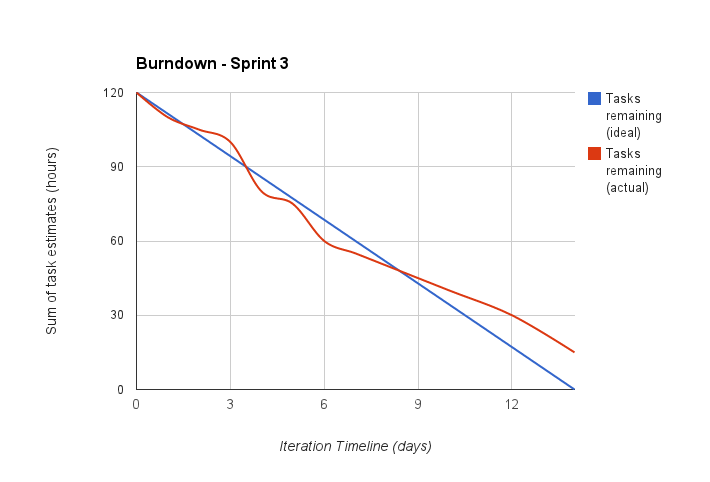
\includegraphics[scale=0.60]{../Figures/burndownSprint3.png}
\caption{Burndown chart Sprint 3}
\label{figure:burndownsprint3}
\end{figure}

\section{Evaluation}

All in all this sprint was successful.
However, refactoring was an unexpectedly time-consuming task and did not achieve expected results.
Luckily, since all refactoring had been performed on a separte branch on Git, it didn't create
problems as we always had a working branch for development and demonstration purposes.

Furthermore, our colleague in Oslo didn't report the time he spent on the project correclty,
and his contribution was discontinuos because he had begun to work full-time.
Talking with him during an internal meeting, we understood that it would have helped to be specific
about what parts of the report we expected him to write. Being cautious about the matter,
we planned less work for him for the next sprint but we were more explicit about what parts
of the report he should have worked on and encouraged him to track his time appropriately.
We tried to make him feel part of the team and we counted on him.


